\documentclass[conference]{IEEEtran}
\IEEEoverridecommandlockouts
\usepackage{float}
\usepackage{cite}
\usepackage{amsmath,amssymb,amsfonts}
\usepackage{algorithm}
\usepackage{algorithmic}
\usepackage{graphicx}
\usepackage{textcomp}
\usepackage{xcolor}
\usepackage{booktabs}
\usepackage{array}
\usepackage{url}
\usepackage{listings}
\usepackage{hyperref}
\usepackage{tikz}
\usetikzlibrary{shapes.geometric, arrows.meta, positioning, calc}

\lstset{
  basicstyle=\ttfamily\footnotesize,
  breaklines=true,
  frame=single,
  backgroundcolor=\color{gray!10},
  keywordstyle=\color{blue},
  commentstyle=\color{green!50!black},
  stringstyle=\color{red},
}

\def\BibTeX{{\rm B\kern-.05em{\sc i\kern-.025em b}\kern-.08em
    T\kern-.1667em\lower.7ex\hbox{E}\kern-.125emX}}
\raggedbottom
\setlength{\parskip}{0pt}
\setlength{\parsep}{0pt}
\begin{document}

\title{On-Device Voice-Controlled UGV\\
Using MFCC and DTW}

\author{
  \IEEEauthorblockN{Divyansh Maheshwari, Shriyansh Chawda and GVV Sharma}
  \IEEEauthorblockA{
    Department of Electrical Engineering\\
    Indian Institute of Technology, Hyderabad\\
    Kandi, India 502284\\
    gadepall@ee.iith.ac.in
  }
}

\maketitle

\begin{abstract}
This paper presents a cloud-free voice-controlled Unmanned Ground
Vehicle (UGV) that performs all speech recognition on an Android
smartphone. The phone records 1.5\,s of audio, extracts
26-dimensional Mel-Frequency Cepstral Coefficient (MFCC) features,
and applies Dynamic Time Warping (DTW) with Best-of-$N$ template
matching (up to $N=10$ templates per command) to identify one of five commands: \textit{forward},
\textit{back}, \textit{left}, \textit{right}, and \textit{stop}.
The recognized command is sent as a 7-byte string over Bluetooth
Low Energy (BLE) to an ESP32, which drives a differential-drive
chassis via an L293D motor driver. Moving recognition off the ESP32
reduces latency from 2--4\,s to 1.6\,s and frees 80\,kB of flash.
User adaptation is supported through up to ten recorded templates
per command, achieving 90--95\% accuracy across 10 speakers and demonstrating
language-agnostic operation in English, Hindi, Gujarati, and Tamil.
\end{abstract}

\begin{IEEEkeywords}
UGV, voice control, MFCC, DTW, ESP32, BLE, Android, speech recognition,
embedded systems
\end{IEEEkeywords}

\section{Introduction} \label{sec:intro}

Voice-based control of robotic platforms provides an intuitive
human--machine interface, eliminating the need for dedicated hardware
controllers. Prior work on speech-driven robots has largely relied on
cloud-based automatic speech recognition (ASR) services, which
introduce network latency, require continuous internet connectivity,
and raise data-privacy concerns \cite{li2017speech}. On the other hand,
running full ASR models directly on low-power microcontrollers has been
constrained by limited memory and compute resources.

Template-based approaches such as Dynamic Time Warping offer a practical
middle ground: they are computationally light, require no training data
beyond a small set of recorded templates, and run entirely on-device.
DTW has been widely used in isolated word recognition \cite{sakoe1978dtw},
and MFCC features are the standard front-end for speech systems \cite{davis1980mfcc}.
Prior work on embedded keyword spotting has shown that neural approaches
can be deployed on microcontrollers \cite{zhang2017hello, choi2019iot}, but
require substantially more training data and memory than the template-based
method presented here. BLE has been established as an effective low-power
communication link for small robotic platforms \cite{mikhaylov2013ble}.

This work places MFCC extraction and DTW matching on an Android
smartphone, exploiting its significantly more powerful processor (compared to the ESP32) and
microphone, while the ESP32 microcontroller is reserved for motor
control and BLE communication. The contribution of this paper is
threefold:
\begin{enumerate}
  \item A fully on-device, cloud-free voice recognition pipeline running
    on a commodity Android phone.
  \item A Best-of-N DTW strategy enabling user adaptation with up to
    ten templates per command.
  \item A latency-optimized BLE communication scheme transmitting only
    a 7-byte command string instead of raw audio frames, reducing the
    BLE payload by over 99\%.
\end{enumerate}

\section{System Architecture} \label{sec:architecture}

\subsection{Overview}
The system comprises two hardware nodes connected via BLE: an Android
smartphone acting as the sensing and recognition unit, and an ESP32
microcontroller acting as the motion controller.

Initially, MFCC extraction and DTW matching were executed directly on
the ESP32. However, this consumed $\sim$80\,kB of flash, required
transferring 24{,}000 bytes of raw audio over BLE before processing,
and introduced 2--4\,s of latency. Migrating the recognition pipeline
to the Android phone reduces the BLE payload to a 7-byte command
string and end-to-end latency to $\sim$1.6\,s, while the ESP32 is
reserved solely for BLE reception and motor control.

\begin{table}[H]
\caption{Architecture Comparison: Old vs.\ New Pipeline}
\centering
\begin{tabular}{lll}
\toprule
\textbf{Stage} & \textbf{Old} & \textbf{New} \\
\midrule
Audio capture      & ESP32 mic          & Android mic    \\
MFCC extraction    & ESP32 (C++)        & Android (Java) \\
DTW matching       & ESP32 (C++)        & Android (Java) \\
BLE payload        & 24{,}000 bytes     & 7 bytes        \\
ESP32 flash        & $\sim$80\,kB extra & Minimal        \\
End-to-end latency & 2--4\,s            & $\sim$1.6\,s   \\
\bottomrule
\end{tabular}
\label{tab:arch}
\end{table}

\subsection{Data Flow}
The complete pipeline proceeds as follows:
\begin{enumerate}
  \item The Android app records 1.5\,s of audio at 8\,kHz mono
    (12{,}000 samples, 16-bit PCM) on button press.
  \item \texttt{MFCCProcessor} extracts a $92 \times 26$ feature matrix
    (13 raw + 13 delta MFCC coefficients per frame).
  \item \texttt{DTWMatcher} computes the Best-of-N DTW score against all
    stored templates for each of the five commands.
  \item If the minimum score is below the acceptance threshold
    ($\tau = 12.0$), the command string is sent over BLE.
  \item The ESP32 receives the string and actuates the motors via the
    L293D driver.
\end{enumerate}

\begin{figure}[H]
\centering
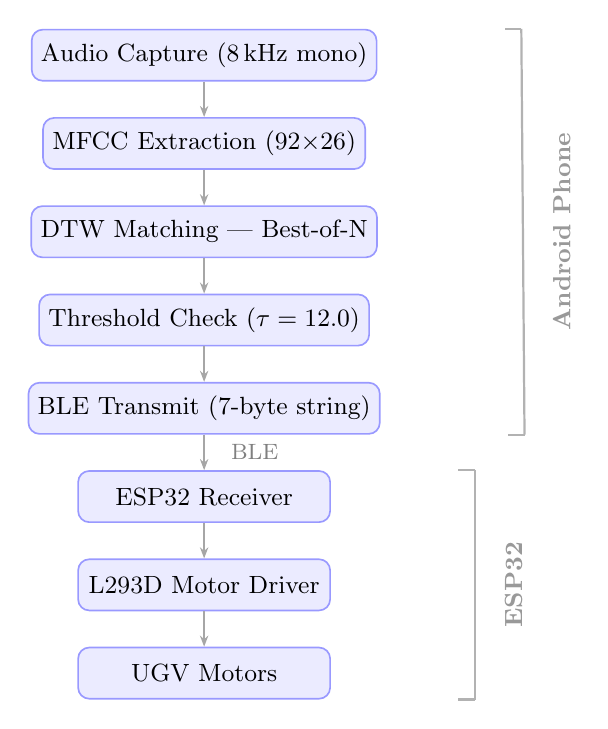
\begin{tikzpicture}[
  node distance=0.45cm,
  block/.style={rectangle, draw, rounded corners=4pt,
    minimum width=3.2cm, minimum height=0.65cm,
    text centered, font=\small, fill=blue!8, draw=blue!40,
    line width=0.6pt},
  arrow/.style={-{Stealth[length=4pt]}, thick, draw=gray!70}
]

\node (audio)  [block]                  {Audio Capture (8\,kHz mono)};
\node (mfcc)   [block, below=of audio]  {MFCC Extraction ($92{\times}26$)};
\node (dtw)    [block, below=of mfcc]   {DTW Matching --- Best-of-N};
\node (thresh) [block, below=of dtw]    {Threshold Check ($\tau = 12.0$)};
\node (ble)    [block, below=of thresh] {BLE Transmit (7-byte string)};
\node (esp)    [block, below=of ble]    {ESP32 Receiver};
\node (motor)  [block, below=of esp]    {L293D Motor Driver};
\node (ugv)    [block, below=of motor]  {UGV Motors};

\draw[arrow] (audio)  -- (mfcc);
\draw[arrow] (mfcc)   -- (dtw);
\draw[arrow] (dtw)    -- (thresh);
\draw[arrow] (thresh) -- (ble);
\draw[arrow] (ble)    -- (esp)
  node[midway, right=6pt, font=\footnotesize, text=gray] {BLE};
\draw[arrow] (esp)    -- (motor);
\draw[arrow] (motor)  -- (ugv);

\draw[thick, gray!60]
  ([xshift=52pt]audio.north east) -- ([xshift=52pt]ble.south east);
\draw[thick, gray!60]
  ([xshift=52pt]audio.north east) -- ([xshift=46pt]audio.north east);
\draw[thick, gray!60]
  ([xshift=52pt]ble.south east)   -- ([xshift=46pt]ble.south east);
\node[font=\small\bfseries, rotate=90, anchor=center, text=gray!80]
  at ([xshift=66pt]$(audio.north east)!0.5!(ble.south east)$)
  {Android Phone};

\draw[thick, gray!60]
  ([xshift=52pt]esp.north east) -- ([xshift=52pt]ugv.south east);
\draw[thick, gray!60]
  ([xshift=52pt]esp.north east) -- ([xshift=46pt]esp.north east);
\draw[thick, gray!60]
  ([xshift=52pt]ugv.south east) -- ([xshift=46pt]ugv.south east);
\node[font=\small\bfseries, rotate=90, anchor=center, text=gray!80]
  at ([xshift=66pt]$(esp.north east)!0.5!(ugv.south east)$)
  {ESP32};

\end{tikzpicture}
\caption{System pipeline block diagram.}
\label{fig:blockdiagram}
\end{figure}

\section{Hardware Setup} \label{sec:hardware}

\subsection{Components}

\begin{table}[H]
\caption{List of Components}
\centering
\begin{tabular}{lll}
\toprule
\textbf{Component}       & \textbf{Qty.} & \textbf{Description} \\
\midrule
Chassis frame            & 1  & Holds all components \\
Side wheels (DC motors)  & 2  & Drive wheels \\
Caster wheel             & 1  & Stability and smooth turning \\
ESP32 dev board          & 1  & Microcontroller + BLE \\
L293D motor driver IC    & 1  & Drives DC motors \\
DC motors (TT gear)      & 2  & Propulsion \\
Breadboard               & 1  & Circuit connections \\
Jumper wires             & 11 & Electrical connections \\
Power bank / LiPo        & 1  & Portable power supply \\
Android phone (API 23+)  & 1  & Recognition + BLE central \\
Micro-USB / USB-C cable  & 1  & ESP32 flashing \\
\bottomrule
\end{tabular}
\label{tab:components}
\end{table}

\begin{figure}[H]
\centering
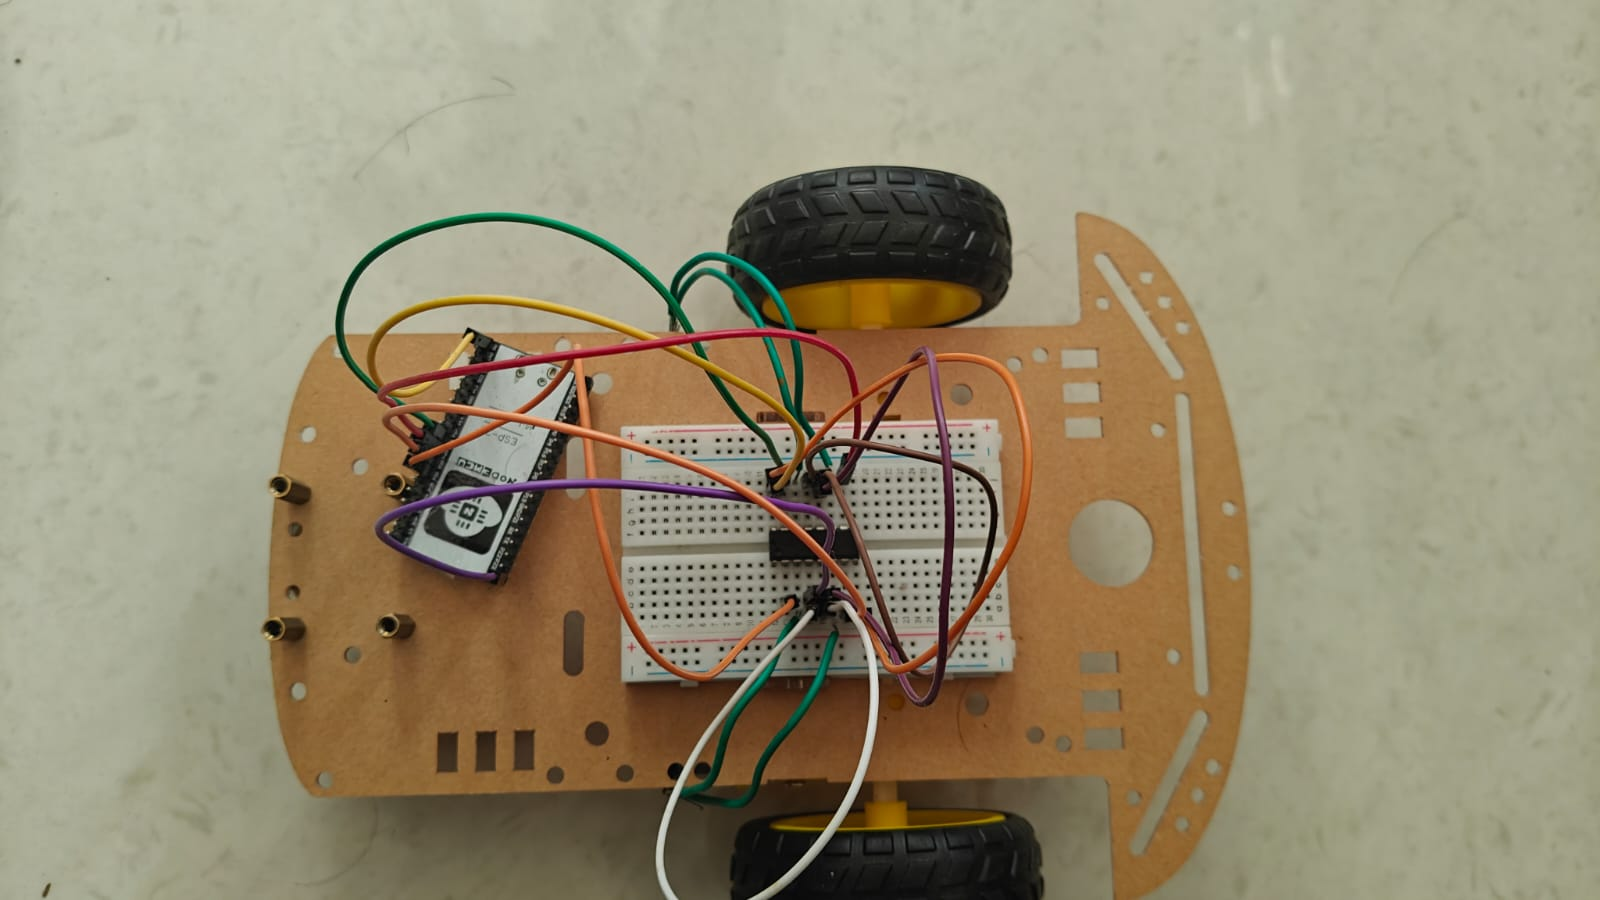
\includegraphics[width=0.8\columnwidth]{figs/ugv_hardware.jpeg} 
\caption{Top-down view of the assembled UGV prototype, detailing the ESP32, breadboard, L293D motor driver, and chassis wiring.}
\label{fig:hardware_setup}
\end{figure}

\subsection{Motor Wiring}

The ESP32 controls the L293D via four digital GPIO pins. The enable pins
EN1 and EN2 of the L293D are wired permanently HIGH.

\begin{table}[htbp]
\caption{ESP32 to L293D Connections}
\centering
\begin{tabular}{ccl}
\toprule
\textbf{ESP32 GPIO} & \textbf{L293D Pin} & \textbf{Function} \\
\midrule
GPIO 32 & IN1      & Motor A --- direction 1 \\
GPIO 33 & IN2      & Motor A --- direction 2 \\
GPIO 25 & IN3      & Motor B --- direction 1 \\
GPIO 26 & IN4      & Motor B --- direction 2 \\
GND     & GND      & Common ground \\
3.3\,V  & EN1, EN2 & Motor channel enable (HIGH) \\
\bottomrule
\end{tabular}
\label{tab:wiring}
\end{table}

\subsection{Full Schematic}
\begin{figure}[H]
\centering
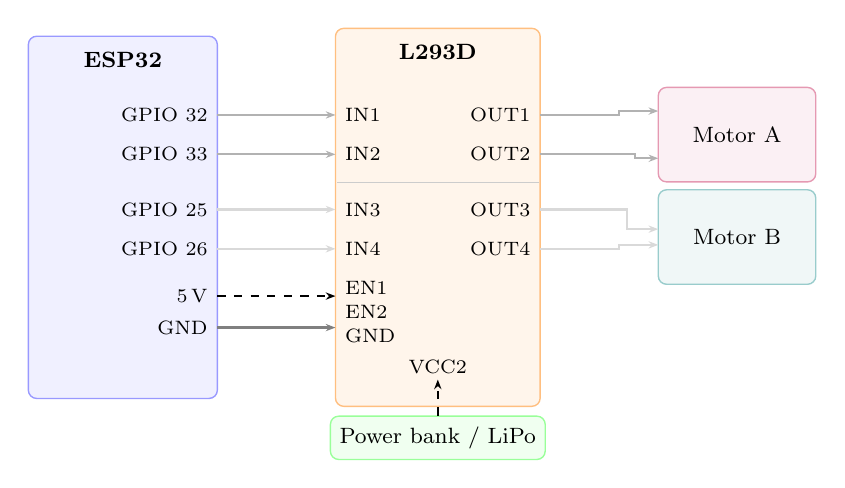
\begin{tikzpicture}[
  node distance=0cm,
  block/.style={rectangle, draw, rounded corners=3pt,
    minimum width=2.2cm, font=\footnotesize,
    text centered, line width=0.5pt},
  pin/.style={font=\scriptsize},
  arrA/.style={-{Stealth[length=3.5pt]}, thick, draw=gray!60},
  arrB/.style={-{Stealth[length=3.5pt]}, thick, draw=gray!30},
  pwr/.style={-{Stealth[length=3.5pt]}, thick, draw=black, dashed},
  gnd/.style={-{Stealth[length=3.5pt]}, thick, draw=black!50},
]

\node[block, fill=blue!6, draw=blue!40,
      minimum width=2.4cm, minimum height=4.6cm]
      (esp) at (0,0) {};
\node[font=\footnotesize\bfseries] at (0, 2.0) {ESP32};

\foreach \lbl/\y in {
  GPIO 32/1.3, GPIO 33/0.8,
  GPIO 25/0.1, GPIO 26/-0.4,
  5\,V/-1.0, GND/-1.4}{
  \node[pin, anchor=east] at (1.2, \y) {\lbl};
}

\node[block, fill=orange!8, draw=orange!50,
      minimum width=2.6cm, minimum height=4.8cm]
      (ic) at (4.0,0) {};
\node[font=\footnotesize\bfseries] at (4.0, 2.1) {L293D};

\foreach \lbl/\y in {
  IN1/1.3, IN2/0.8, IN3/0.1, IN4/-0.4,
  EN1/-0.9, EN2/-1.2, GND/-1.5}{
  \node[pin, anchor=west] at (2.7, \y) {\lbl};
}

\foreach \lbl/\y in {OUT1/1.3, OUT2/0.8, OUT3/0.1, OUT4/-0.4}{
  \node[pin, anchor=east] at (5.3, \y) {\lbl};
}
\node[pin] at (4.0,-1.9) {VCC2};

\draw[gray!40, thin] (2.72, 0.44) -- (5.28, 0.44);

\node[block, fill=purple!6, draw=purple!40,
      minimum width=2.0cm, minimum height=1.2cm]
      (ma) at (7.8, 1.05) {Motor A};

\node[block, fill=teal!6, draw=teal!40,
      minimum width=2.0cm, minimum height=1.2cm]
      (mb) at (7.8,-0.25) {Motor B};

\node[block, fill=green!6, draw=green!40,
      minimum width=2.6cm, minimum height=0.55cm]
      (pwr) at (4.0,-2.8) {Power bank / LiPo};

\draw[arrA] (1.2, 1.3) -- (2.7, 1.3);
\draw[arrA] (1.2, 0.8) -- (2.7, 0.8);
\draw[arrB] (1.2, 0.1) -- (2.7, 0.1);
\draw[arrB] (1.2,-0.4) -- (2.7,-0.4);
\draw[pwr] (1.2,-1.0) -- (2.7,-1.0);
\draw[gnd] (1.2,-1.4) -- (2.7,-1.4);

\draw[pwr] (4.0,-2.52) -- (4.0,-2.06);

\draw[arrA] (5.3, 1.3) -| (6.3, 1.35) -- (6.8, 1.35);
\draw[arrA] (5.3, 0.8) -| (6.5, 0.75) -- (6.8, 0.75);

\draw[arrB] (5.3, 0.1) -| (6.4,-0.15) -- (6.8,-0.15);
\draw[arrB] (5.3,-0.4) -| (6.3,-0.35) -- (6.8,-0.35);

\end{tikzpicture}
\caption{Wiring schematic: ESP32 to L293D to DC motors.
  Dark arrows — Motor A channel (GPIO\,32/33 $\to$ IN1/IN2 $\to$ OUT1/OUT2).
  Light arrows — Motor B channel (GPIO\,25/26 $\to$ IN3/IN4 $\to$ OUT3/OUT4).
  Dashed — power connections (3.3\,V to EN1, EN2; motor supply to VCC2).}
\label{fig:wiring}
\end{figure}

\subsection{Motor Truth Table}

\begin{table}[htbp]
\caption{Motor Direction Truth Table}
\centering
\begin{tabular}{ccccl}
\toprule
\textbf{IN1} & \textbf{IN2} & \textbf{IN3} & \textbf{IN4} & \textbf{Result} \\
\midrule
H & L & H & L & Move Forward \\
L & H & L & H & Move Back    \\
L & H & H & L & Turn Left    \\
H & L & L & H & Turn Right   \\
L & L & L & L & Motor Stop   \\
\bottomrule
\end{tabular}
\label{tab:truth}
\end{table}

\section{Signal Processing --- MFCC Feature Extraction} \label{sec:mfcc}

MFCC extraction transforms raw audio into a compact, speaker-adapted
feature representation. The full mathematical derivation of each stage
is given in Appendix~\ref{app:math}; the pipeline follows seven
sequential stages.

\subsection{Framing Parameters}
Audio is segmented into overlapping frames: frame size $N = 256$ samples
(32\,ms at 8\,kHz), hop size $H = 128$ samples (16\,ms, 50\% overlap),
giving $(12000 - 256)/128 + 1 = 92$ frames for a 1.5\,s recording.

\subsection{Pre-emphasis}
A first-order high-pass filter ($\alpha = 0.97$) boosts high-frequency
content (Eq.~\ref{eq:preemphasis}). The signal is normalized to
$[-1, 1]$ by dividing by 32768 prior to windowing.

\subsection{Hamming Window}
Each frame is multiplied by a Hamming window (Eq.~\ref{eq:hamming})
to reduce spectral leakage.

\subsection{Fast Fourier Transform and Power Spectrum}
A 256-point radix-2 Cooley--Tukey FFT is applied. The one-sided power
spectrum (Eq.~\ref{eq:powspec}) retains the first $N/2 + 1 = 129$ bins.

\subsection{Mel Filterbank}
The Mel scale (Eq.~\ref{eq:meltohz}) maps frequency to a perceptually
uniform scale. Twenty-six triangular filters equally spaced on the Mel
scale are applied to the power spectrum, and log energy is computed per
filter (Eq.~\ref{eq:melbank}). A floor of $10^{-10}$ prevents $\log(0)$.

\subsection{Discrete Cosine Transform}
DCT-II with orthonormal normalization (Eqs.~\ref{eq:dct}--\ref{eq:dctweight})
decorrelates the 26 log-energies into 13 MFCC coefficients.

\subsection{Delta Coefficients}
Delta (velocity) features (Eq.~\ref{eq:delta}) capture temporal dynamics
and are appended to each frame, doubling the feature dimension from 13
to 26. Edge frames use the nearest valid neighbor.

\subsection{Cepstral Mean and Variance Normalisation (CMVN)}
CMVN (Eqs.~\ref{eq:mean}--\ref{eq:cmvn}) removes channel effects and
normalizes each coefficient across all frames, where
$\varepsilon = 10^{-8}$ prevents division by zero.
The final MFCC output is a matrix of shape $92 \times 26$, representing
92 frames each with 26 normalized coefficients.

\section{Pattern Matching --- Dynamic Time Warping} \label{sec:dtw}
\subsection{DTW Algorithm}
Given a query sequence $\mathbf{Q}$ of length $F_1$ and a template
$\mathbf{T}$ of length $F_2$, each with 26-dimensional feature vectors,
DTW finds the optimal non-linear alignment using Euclidean distance
(Eq.~\ref{eq:euclid}). The accumulated cost matrix is filled by the
recurrence in Eq.~\ref{eq:dtw}. A parallel path-length matrix $L$
(Eq.~\ref{eq:pathlen}) tracks steps along the warping path, and the
final normalized DTW score (Eq.~\ref{eq:dtwnorm}) removes the bias
introduced by different word durations. Memory usage is reduced from
$O(F_1 F_2)$ to $O(F_2)$ by maintaining only two rolling rows of
$D$ and $L$. Full derivations are given in Appendix~\ref{app:math}.

\subsection{Best-of-N Strategy}
Each command stores up to $N=10$ templates (index 0 from the original
trained header, indices 1--9 recorded in-app). The command score is the
minimum DTW score across all stored templates (Eq.~\ref{eq:bestofn}).
Recognition proceeds by selecting the command with the lowest score,
subject to an acceptance threshold $\tau$ (Eq.~\ref{eq:decision}).
The default threshold is $\tau = 12.0$. Table~\ref{tab:results}
summarises the interpretation of DTW scores observed in practice.
\section{Recognition Algorithm} \label{sec:recognition}

This section presents the complete end-to-end voice recognition pipeline as
formal algorithms. Algorithm~\ref{alg:mfcc} describes MFCC feature extraction,
and Algorithm~\ref{alg:dtw} describes the DTW-based command recognition with
Best-of-N template matching.
% \vspace{-30pt}
\begin{algorithm}[H]
\caption{MFCC Feature Extraction}
\label{alg:mfcc}
\begin{algorithmic}[1]
\REQUIRE Raw audio samples $x[n]$, $n=0,\ldots,11999$ (1.5\,s at 8\,kHz)
\ENSURE Feature matrix $\hat{\mathbf{C}} \in \mathbb{R}^{92 \times 26}$

\STATE \textbf{Pre-emphasis:} $y[n] \leftarrow x[n] - 0.97\,x[n-1]$; normalize by $32768$
\FOR{each frame $f = 0$ \TO $91$}
  \STATE Extract samples $y[fH : fH+N]$ with $N=256$, $H=128$
  \STATE Apply Hamming window: $s[n] \leftarrow y[n]\cdot w[n]$
  \STATE Compute 256-point FFT; form power spectrum $P[k] = |X[k]|^2/N$
  \STATE Apply 26-band Mel filterbank; compute log energies $E[m]$
  \STATE Apply DCT-II to $E[m]$; retain first 13 coefficients $\mathbf{c}[f]$
\ENDFOR
\FOR{each frame $f = 0$ \TO $91$}
  \STATE Compute delta: $\Delta c[f][k] \leftarrow (c[f{+}1][k] - c[f{-}1][k])/2$
  \STATE Concatenate: $\mathbf{c}[f] \leftarrow [\mathbf{c}[f] \;\|\; \Delta\mathbf{c}[f]]$ (26-dim)
\ENDFOR
\STATE Compute per-coefficient mean $\mu_k$ and std $\sigma_k$ across all frames
\STATE CMVN: $\hat{c}[f][k] \leftarrow (c[f][k] - \mu_k)/(\sigma_k + 10^{-8})$
\RETURN $\hat{\mathbf{C}}$
\end{algorithmic}
\end{algorithm}
\vspace{-16pt}
\begin{algorithm}[H]
\caption{Voice Command Recognition via DTW + Best-of-N}
\label{alg:dtw}
\begin{algorithmic}[1]
\REQUIRE Query MFCC matrix $\mathbf{Q} \in \mathbb{R}^{F_1 \times 26}$,
         template sets $\{\mathbf{T}_{c,i}\}$ for each command $c$,
         threshold $\tau = 12.0$
\ENSURE Recognized command $\hat{c}$, or \textsc{reject}

\FOR{each command $c \in \{$\textit{forward, back, left, right, stop}$\}$}
  \STATE $s_c \leftarrow \infty$
  \FOR{each stored template $\mathbf{T}_{c,i}$ of length $F_2$}
    \STATE Initialize $D_{\text{prev}}[j] \leftarrow \infty$,
           $L_{\text{prev}}[j] \leftarrow 0$ for $j=0,\ldots,F_2{-}1$
    \FOR{$i = 0$ \TO $F_1 - 1$}
      \FOR{$j = 0$ \TO $F_2 - 1$}
        \STATE $d \leftarrow \|\mathbf{Q}[i] - \mathbf{T}_{c,i}[j]\|_2$
        \STATE $p^* \leftarrow \arg\min(D[i{-}1][j],\,D[i][j{-}1],\,D[i{-}1][j{-}1])$
        \STATE $D_{\text{curr}}[j] \leftarrow d + D_{p^*}$;\quad
               $L_{\text{curr}}[j] \leftarrow 1 + L_{p^*}$
      \ENDFOR
      \STATE $D_{\text{prev}} \leftarrow D_{\text{curr}}$;\quad
             $L_{\text{prev}} \leftarrow L_{\text{curr}}$
    \ENDFOR
    \STATE $\text{score} \leftarrow D_{\text{prev}}[F_2{-}1]\,/\,L_{\text{prev}}[F_2{-}1]$
    \STATE $s_c \leftarrow \min(s_c,\;\text{score})$ \hfill\COMMENT{Best-of-N}
  \ENDFOR
\ENDFOR
\STATE $\hat{c} \leftarrow \arg\min_c\; s_c$
\IF{$s_{\hat{c}} < \tau$}
  \RETURN $\hat{c}$
\ELSE
  \RETURN \textsc{reject}
\ENDIF
\end{algorithmic}
\end{algorithm}

\section{Software Implementation} \label{sec:software}

\subsection{ESP32 Firmware}

The firmware is written in C++ using the Arduino framework and built
with PlatformIO. It contains three source files.

\textbf{ble\_receive.cpp} implements a BLE GATT server with two
characteristics: a WRITE characteristic
(\texttt{UUID:~...9002}) for receiving command strings, and a NOTIFY
characteristic (\texttt{UUID:~...9003}) for sending acknowledgements.
Only the five known command strings are accepted; all other writes are
silently discarded. On client disconnect, BLE advertising restarts
automatically.

\textbf{motor.cpp} drives the L293D via four GPIO pins (32, 33, 25, 26)
using simple digital writes. No PWM speed control is used.

\textbf{main.cpp} implements the command dispatcher:

\begin{lstlisting}[language=C++, caption={ESP32 command dispatcher (main.cpp)}]
void loop() {
  char cmd[16] = {0};
  if (!ble_receive_command(cmd, sizeof(cmd)))
    { delay(5); return; }

  if      (!strcmp(cmd,"forward")) { motor_forward(); }
  else if (!strcmp(cmd,"back"))    { motor_back(); }
  else if (!strcmp(cmd,"left"))
    { motor_left();  delay(600); motor_stop(); }
  else if (!strcmp(cmd,"right"))
    { motor_right(); delay(600); motor_stop(); }
  else if (!strcmp(cmd,"stop"))    { motor_stop(); }
}
\end{lstlisting}

\textit{forward} and \textit{back} run continuously until a \textit{stop}
command is received. \textit{left} and \textit{right} execute for 600\,ms
then auto-stop, producing approximately a 90° turn. The turn duration
is tunable to adjust the turning angle.

\subsection{Android Application}
The Android app records 1.5\,s of audio at 8\,kHz mono, extracts
MFCC features, and runs DTW matching entirely on-device. All
processing runs on a background thread, with results delivered to
the UI thread on completion. If the best DTW score falls below the
threshold $\tau$, the command string is written to the BLE
characteristic. The app also provides a debug screen showing live
DTW scores per command and a training interface for recording
additional templates. A 200\,ms delay before each \texttt{AudioRecord}
initialisation prevents microphone release errors on rapid consecutive
recordings.

\subsection{Template Conversion Script}
A one-time Python script (\texttt{convert\_templates.py}) converts the
C header \texttt{templates.h} — which stores the original trained
MFCC templates as float arrays — into the binary \texttt{.bin} format
consumed by \texttt{TemplateStore}. The script uses a regular expression
to locate each template array and its frame-count \texttt{\#define},
strips the C-style \texttt{f} suffix from float literals, and writes
the binary file with \texttt{struct.pack}.

\subsection{Out-of-the-Box Deployment}
A key advantage of this architecture is its straightforward deployment. By directly uploading the provided C++ firmware to the ESP32 and installing the companion APK on an Android device, the system requires minimal configuration. The ESP32 is configured with a fixed MAC address matching the one expected by the application. Therefore, once the user manually pairs the ESP32 with their smartphone via the standard Android Bluetooth settings, the UGV becomes fully operational. The user can then simply open the app, speak a command, and the vehicle will respond promptly (within approximately 1.6\,s).

\section{User Adaptation and Tuning} \label{sec:tuning}

\subsection{Recording Additional Templates}

Template index 0 (loaded from \texttt{assets}) is the original trained
template. Indices 1--9 are recorded in-app via \texttt{DebugActivity}.
Table~\ref{tab:samples} lists recommended sample counts per scenario.

% NOTE: In tables/table_samples.tex, the row "Multiple speakers — Not supported"
% must be corrected to read "Shared templates across speakers — Not supported"
% to avoid contradicting the multi-speaker evaluation results in Section VIII.
\begin{table}[H]
\caption{Recommended Template Count per Scenario}
\centering
\begin{tabular}{lcc}
\toprule
\textbf{Scenario} & \textbf{Min.} & \textbf{Recommended} \\
\midrule
Quick prototype, quiet room  & 1 & 3--5  \\
Daily driver, single speaker & 5 & 8--10 \\
Noisy environment            & 8 & 10    \\
Shared templates across speakers& \multicolumn{2}{c}{Not supported} \\
\bottomrule
\end{tabular}
\label{tab:samples}
\end{table}

\subsection{Threshold Tuning}

The optimal threshold lies between the highest correct-command score
and the lowest wrong-command score observed in the debug view. With
8--10 templates per command, a threshold of 8.0--10.0 is achievable
for a single speaker in a quiet environment.

\subsection{Turn Duration}

The 600\,ms turn duration in \texttt{main.cpp} is calibrated to produce
approximately 90° on the target chassis at full motor speed. It should
be increased for heavier chassis or slower motors, and decreased for
faster ones.

\section{Results and Discussion} \label{sec:results}

\begin{figure}[t]
\centering
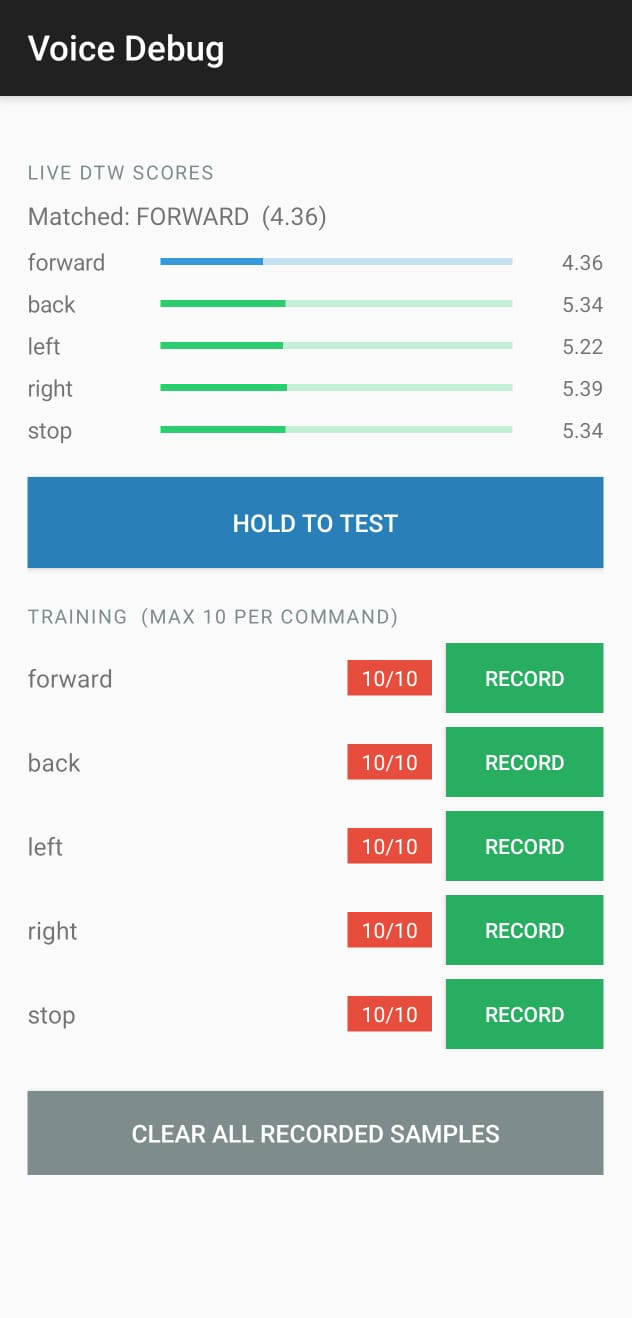
\includegraphics[width=0.62\columnwidth]{figs/debug.png}
\caption{Debug Activity screen showing live DTW scores after speaking
\textit{forward}. The blue bar indicates the winning command (score
4.36), while all other commands score above 5.0. All five commands
have 10 recorded templates (10/10), producing well-separated scores
and reliable recognition.}
\label{fig:debug}
\end{figure}

\subsection{Multi-Speaker Evaluation}
The system was evaluated with \textbf{10 speakers} each recording 10 templates per command using
the in-app training interface. Testing was conducted in a quiet
indoor environment. Overall recognition accuracy across all speakers
and commands was \textbf{90--95\%}, summarised in
Table~\ref{tab:results}.

\begin{table}[H]
\caption{Typical DTW Scores (single speaker, quiet environment)}
\centering
\begin{tabular}{lcc}
\toprule
\textbf{Condition} & \textbf{Score Range} & \textbf{Outcome} \\
\midrule
Correct command, 10 templates & 3.0 -- 7.5   & Match ($<\tau$)      \\
Correct command, 1 template   & 5.0 -- 11.0  & Match / borderline   \\
Wrong command                 & 11.0 -- 22.0 & No match ($>\tau$)   \\
Silent / noise                & 18.0 -- 30.0 & No match             \\
\bottomrule
\end{tabular}
\label{tab:results}
\end{table}

This result is noteworthy because DTW is inherently a
speaker-dependent method --- the base templates were recorded by a
single speaker, yet the system achieved high accuracy across all 10
participants. It should be noted that 10 speakers represents a limited
evaluation cohort; larger-scale testing across more diverse acoustic
conditions is planned as future work. This generalization is attributed to two design
decisions: CMVN normalization (Equation~\ref{eq:cmvn}), which removes
speaker-dependent channel effects from the feature vectors, and the
Best-of-N strategy (Equation~\ref{eq:bestofn}), which allows each
user to personalize recognition with their own recorded templates.

\subsection{Cross-Language Evaluation}
The system was also tested with speakers using commands spoken in
\textbf{Hindi, Gujarati, and Tamil}. Since the recognition pipeline
operates entirely on acoustic features (MFCC + DTW) with no linguistic
model, it is language-agnostic --- any consistent spoken word can
serve as a command regardless of the language it comes from.
Recognition accuracy in the range of 90--95\% was observed across all
tested languages, comparable to the English baseline, further
validating the generality of the approach.

\subsection{Latency}
End-to-end latency was measured at approximately 1.6\,s, compared
to 2--4\,s in the prior architecture where raw audio was streamed
to the ESP32 for processing. The reduction is attributed to
eliminating the 24{,}000-byte BLE audio transfer and replacing it
with a 7-byte command string.

\subsection{Limitations}
The system does not natively support multiple speakers without
per-user template recording. Performance degrades in high-noise
environments, though Android's built-in
\texttt{NoiseSuppressor} API partially mitigates this. Future
work will explore lightweight neural network classifiers and
speaker-independent models deployable on-device.

\section{Conclusions} \label{sec:conclusions}
This paper demonstrated that MFCC feature extraction and DTW pattern
matching can be migrated from a resource-constrained ESP32
microcontroller to a commodity Android smartphone, yielding a
fully on-device, cloud-free voice control pipeline for a UGV.
The architectural shift reduced end-to-end latency from 2--4\,s to
1.6\,s and freed 80\,kB of microcontroller flash, while the
Best-of-$N$ strategy and CMVN normalization together enabled
90--95\% recognition accuracy across 10 speakers and four languages
(English, Hindi, Gujarati, and Tamil) despite DTW being inherently
speaker-dependent.

The current system has two notable limitations: per-user template
recording is required for new speakers, and performance degrades in
high-noise environments. Future work will address these by exploring
lightweight convolutional or recurrent keyword-spotting models
deployable on-device, incorporating data-augmentation to improve
noise robustness, and conducting a larger-scale evaluation across a
broader and more diverse speaker population to provide statistically
robust accuracy estimates.

\nocite{*}
\bibliographystyle{IEEEtran}
\bibliography{references/main}

% NOTE FOR references/main.bib — add the following three entries:
%
% @inproceedings{zhang2017hello,
%   author    = {Y. Zhang and N. Suda and L. Lai and V. Chandra},
%   title     = {Hello Edge: Keyword Spotting on Microcontrollers},
%   year      = {2017},
%   eprint    = {1711.07128},
%   archivePrefix = {arXiv}
% }
%
% @article{choi2019iot,
%   author  = {S. Choi and S. Seo and B. Moon},
%   title   = {An Efficient Keyword Spotting Technique Using a Recurrent
%              Neural Network for Resource-Constrained Devices},
%   journal = {Applied Sciences},
%   volume  = {9},
%   number  = {9},
%   pages   = {1885},
%   year    = {2019}
% }
%
% @inproceedings{mikhaylov2013ble,
%   author    = {K. Mikhaylov and J. Tervonen},
%   title     = {Evaluation of Power Consumption for {B}luetooth Low Energy},
%   booktitle = {Proc. IEEE International Symposium on Personal, Indoor and
%                Mobile Radio Communications (PIMRC)},
%   year      = {2013}
% }

\appendix
\section{Mathematical Derivations}
\label{app:math}

This appendix collects all equations referenced in
Sections~\ref{sec:mfcc} and~\ref{sec:dtw}.

\subsection*{B.1\quad MFCC Feature Extraction}

\textbf{Pre-emphasis:}
\begin{equation}
  y[n] = x[n] - \alpha\, x[n-1], \quad \alpha = 0.97
  \label{eq:preemphasis}
\end{equation}

\textbf{Hamming window:}
\begin{equation}
  w[n] = 0.54 - 0.46\cos\!\left(\frac{2\pi n}{N-1}\right),
  \quad n = 0,\ldots,N-1
  \label{eq:hamming}
\end{equation}

\textbf{Power spectrum:}
\begin{equation}
  P[k] = \frac{|X[k]|^2}{N}, \quad k = 0,\ldots,\frac{N}{2}
  \label{eq:powspec}
\end{equation}

\textbf{Mel scale:}
\begin{equation}
  m = 2595\log_{10}\!\left(1 + \frac{f}{700}\right)
  \label{eq:meltohz}
\end{equation}

\textbf{Mel filterbank log energy:}
\begin{equation}
  E[m] = \log\!\left(\sum_{k} P[k]\,H_m[k]\right),
  \quad m = 0,\ldots,25
  \label{eq:melbank}
\end{equation}

\textbf{DCT-II coefficients:}
\begin{equation}
  c[k] = w_k \sum_{n=0}^{M-1} E[n]
         \cos\!\left(\frac{\pi k (2n+1)}{2M}\right),
  \quad k = 0,\ldots,12
  \label{eq:dct}
\end{equation}
\begin{equation}
  w_k = \begin{cases} \sqrt{1/M} & k=0 \\ \sqrt{2/M} & k>0 \end{cases}
  \label{eq:dctweight}
\end{equation}
where $M = 26$.

\textbf{Delta coefficients:}
\begin{equation}
  \Delta c[f][k] = \frac{c[f{+}1][k] - c[f{-}1][k]}{2}
  \label{eq:delta}
\end{equation}

\textbf{CMVN:}
\begin{align}
  \mu_k     &= \frac{1}{F}\sum_{f=1}^{F} c[f][k] \label{eq:mean}\\
  \sigma_k  &= \sqrt{\frac{1}{F}\sum_{f=1}^{F}
               \bigl(c[f][k]-\mu_k\bigr)^2} \label{eq:std}\\
  \hat{c}[f][k] &= \frac{c[f][k] - \mu_k}{\sigma_k + \varepsilon}
  \label{eq:cmvn}
\end{align}
where $\varepsilon = 10^{-8}$.

\subsection*{B.2\quad Dynamic Time Warping}

\textbf{Local distance:}
\begin{equation}
  d(i,j) = \left\|\mathbf{Q}[i] - \mathbf{T}[j]\right\|_2
  \label{eq:euclid}
\end{equation}

\textbf{Accumulated cost recurrence:}
\begin{equation}
  D[i][j] = d(i,j) + \min\bigl(D[i{-}1][j],\;
             D[i][j{-}1],\; D[i{-}1][j{-}1]\bigr)
  \label{eq:dtw}
\end{equation}

\textbf{Path-length tracking:}
\begin{equation}
  L[i][j] = 1 + L[\,p^*]
  \label{eq:pathlen}
\end{equation}
where $p^* = \arg\min\bigl(D[i{-}1][j],\; D[i][j{-}1],\; D[i{-}1][j{-}1]\bigr)$.

\textbf{Normalized DTW score:}
\begin{equation}
  \text{score} = \frac{D[F_1{-}1][F_2{-}1]}{L[F_1{-}1][F_2{-}1]}
  \label{eq:dtwnorm}
\end{equation}

\textbf{Best-of-N command score:}
\begin{equation}
  s(\text{cmd}) = \min_{i=0}^{N-1} \text{score}(\mathbf{Q},\,\mathbf{T}_i)
  \label{eq:bestofn}
\end{equation}

\textbf{Decision rule:}
\begin{equation}
  \hat{c} = \underset{\text{cmd}}{\arg\min}\; s(\text{cmd}),
  \quad \text{if } \min_{\text{cmd}} s(\text{cmd}) < \tau
  \label{eq:decision}
\end{equation}
\appendix
\section{Software Installation}
\label{app:install}

This appendix provides step-by-step instructions for setting up the
complete development environment, flashing the ESP32 firmware, and
building and installing the Android application.

\subsection*{A.1\quad Prerequisites}

The following tools must be installed on the host PC before proceeding:

\begin{itemize}
  \item \textbf{Python 3.8+} — required for template conversion and
    PlatformIO's build system. Available at \url{https://www.python.org}.
  \item \textbf{Git} — for cloning the repository.
    Available at \url{https://git-scm.com}.
  \item \textbf{VS Code} (recommended) or any editor with PlatformIO support.
\end{itemize}

\subsection*{A.2\quad ESP32 Firmware} \label{app:esp32}

\begin{enumerate}
  \item \textbf{Install PlatformIO.}
    Install the PlatformIO IDE extension in VS Code, or install the
    PlatformIO Core CLI via:
\begin{lstlisting}[language=bash]
pip install platformio
\end{lstlisting}

  \item \textbf{Clone / extract the project.}
    Place the \texttt{ugv\_esp32/} folder on your PC.

  \item \textbf{Generate MFCC template binaries.}
    Run the conversion script once to produce the \texttt{.bin} files
    consumed by the Android app:
\begin{lstlisting}[language=bash]
cd ugv_esp32
python convert_templates.py
\end{lstlisting}
    This reads \texttt{templates.h} and writes one binary file per
    command into the \texttt{assets/} folder.

  \item \textbf{Connect the ESP32} to the PC via USB.

  \item \textbf{Build and flash} the firmware:
\begin{lstlisting}[language=bash]
pio run --target upload
\end{lstlisting}
    PlatformIO automatically installs the \texttt{ESP32 BLE Arduino}
    library declared in \texttt{platformio.ini}.
    After flashing, the ESP32 advertises itself as \texttt{ESP32\_UGV}
    over BLE and awaits a connection.

  \item \textbf{Verify} by opening the serial monitor
    (\texttt{pio device monitor}, 115200\,baud) and confirming the
    message \texttt{BLE started, advertising...}.
\end{enumerate}

\subsection*{A.3\quad Android Application} \label{app:android}

\subsubsection*{Option A — Install the pre-built APK (recommended)}
\begin{enumerate}
  \item Copy \texttt{ugv\_android.apk} to the Android device.
  \item On the device, enable \textit{Settings $\to$ Security $\to$
    Install unknown apps} for your file manager.
  \item Open the APK file and tap \textit{Install}.
\end{enumerate}

\subsubsection*{Option B — Build from source with Android Studio}
\begin{enumerate}
  \item \textbf{Install Android Studio} (Hedgehog or later) from
    \url{https://developer.android.com/studio}.
    During setup, install the Android SDK (API level 33+) and
    the Android NDK if prompted.

  \item \textbf{Open the project.}
    In Android Studio, choose \textit{File $\to$ Open} and select the
    \texttt{ugv\_android/} folder. Wait for Gradle sync to complete.

  \item \textbf{Copy template assets.}
    Paste the \texttt{.bin} files generated in Section~A.2 Step~3 into:
\begin{lstlisting}
ugv_android/app/src/main/assets/
\end{lstlisting}

  \item \textbf{Build the APK.}
    Select \textit{Build $\to$ Build Bundle(s) / APK(s) $\to$
    Build APK(s)}. The signed debug APK is placed in:
\begin{lstlisting}
app/build/outputs/apk/debug/app-debug.apk
\end{lstlisting}

  \item \textbf{Deploy to device.}
    Connect an Android phone (USB debugging enabled), then click
    \textit{Run $\to$ Run 'app'} or use:
\begin{lstlisting}[language=bash]
adb install app/build/outputs/apk/debug/app-debug.apk
\end{lstlisting}
\end{enumerate}

\subsection*{A.4\quad First-Time Setup on the Phone}

\begin{enumerate}
  \item Enable Bluetooth on the Android device.
  \item Open the \textbf{UGV Controller} app.
    The \textit{SetupActivity} wizard launches automatically on first
    run, guiding you through BLE pairing.
  \item Tap \textit{Connect to ESP32}. The app scans for a BLE device
    named \texttt{ESP32\_UGV} and connects automatically.
  \item Follow the on-screen prompts to record 5 templates per command
    (10 recommended for best accuracy).
  \item Tap any command button to issue voice commands. The recognized
    command and DTW score are shown on the main screen; detailed
    per-command scores are available in the \textit{Debug} screen.
\end{enumerate}

\subsection*{A.5\quad Troubleshooting}

\begin{itemize}
  \item \textbf{AudioRecord failed:} A 200\,ms delay is already applied
    between recordings. If the error persists, close other apps
    using the microphone.
  \item \textbf{BLE not connecting:} Ensure the ESP32 is powered and
    advertising (\texttt{ESP32\_UGV} appears in a BLE scanner app).
    Force-stop the UGV app and reconnect.
  \item \textbf{Poor recognition accuracy:} Record additional templates
    in a quiet environment. Reduce the threshold $\tau$ in
    \texttt{DTWMatcher.java} if valid commands are being rejected.
  \item \textbf{Gradle build errors:} Ensure JDK 17 is selected in
    \textit{File $\to$ Project Structure $\to$ SDK Location}.
\end{itemize}

\end{document}
